\chapter{Developer documentation}
\label{ch:impl}

This chapter will offer insight into the project's development and implementation structure, design and extensibility. It will provide developers with a comprehensive understanding of the technology stack and functionality. This resource enables contributions, enhancements, and future development leveraging the project's components.

\section{Development Tools}\label{sec:dev_tools}
The \href{https://github.com/aamnatayyab6/StudyBuddy_FE.git}{frontend} and \href{https://github.com/mastertimisensei/StudyBuddyBE.git}{backend} repositories of the project can be forked, built and tested on GitHub.
This application is developed using React Native (0.71.7) and Expo (SDK Version 48.0.10). The following tools provide a comprehensive overview of the development environment:
\begin{itemize}
    \item Android Version 5+: Expo SDK Version 48.0.10 supports minimum SDK version 21 for Android which means that all versions after 21 can compile the application.
    \item Target Version: the compileSdkVersion is 33 for Expo SDK Version 48.0.0+ \cite{ExpoDoc}
    \item Expo Command Line Interface (CLI) that serves as the primary interface between developer and other Expo tools.
    \item To use Expo CLI one needs to have the following tools on the developer machine:
    \begin{itemize}
        \item Node.js 
        \item Git
    \end{itemize}
    \item Visual Studio Code (or any preferred code editor).
    \item Expo Go Client App installed on your emulator or physical device (only for testing because it is not needed to build anything locally with Expo Go).
\end{itemize}
The development tools specific to the development of this app and the reasons of these choices are mentioned in the next Section \ref{sec:guidelines}.
\section{Development Guidelines}\label{sec:guidelines}
\subsection{Strategy}
The front-end development strategy for this application focused on creating a cross platform application and an intuitive user experience built using windows operating system which turned out to be limitation during development later as mentioned in Section \ref{sec:constraints}. To achieve this, a combination of carefully chosen tools and technology was employed. These tools played a vital role in shaping the app's design, functionality, and overall front-end development process. The following tools were utilized during the front-end development, chosen for their specific capabilities and benefits also mentioned below:
\begin{itemize}
    \item React Native (0.71.7) and Expo (SDK Version 48.0.10): React Native is a cross-platform library that builds native mobile apps. It inherits all the functionalities from the popular web framework ReactJS. Expo is a framework that is used to build React Native apps. This comprehensive toolkit consists of various tools and services specifically designed for React Native. Expo was selected for several compelling reasons, including its ability to facilitate rapid development, handle native code complexities under the hood, eliminate the need for direct Android Studio involvement, provide Over-The-Air (OTA) updates, and offer the advantages of being a free and open-source framework. \cite{hutri2023comparison}
    \item Expo Command Line Interface (CLI) version 6.3.2.
    \item Node.js version 16.19.1 installed with npm version 8.19.3.
    \item Git version 2.33.1.windows.1.
    \item JDK 17.0.6 for generating apk.
    \item Visual Studio Code editor with useful extensions such as Tabnine, Expo Tools, and TailwindCSS.
    \item Expo Go Client App installed on Android 11 (API 30) emulator.
\end{itemize}
\subsection{Codebase Organization}
There are organized directories and files in the codebase to enhance readability, maintainability, and collaboration. Here is a description of the structure of the codebase for the front-end of the project:
\begin{compactenum}
    \item \textbf{Root Directory:} 
    \begin{itemize}
        \item App.js: The main entry point of the application.
        \item Config files: Various configuration files such as app.json, babel.config.js, package-lock.json, package.json, and tailwind.config.json. These files define project settings, dependencies, and build configurations.
    \end{itemize}
    \item \textbf{Src Folder:}
    \begin{itemize}
        \item Assets: Contains the images folder, where images used in the application are stored.
        \item Const: Includes files that hold reusable data that remains constant throughout the project, such as styles.js for custom styling, slides.js for onboarding slider information, colors.js for defining color schemes, and placeholder\_image\_uri.js for placeholder image URL.
        \item api: Contains UserContext.js, a custom hook for managing context API state and functionality. It also contains Storage.js for managing Async Storage used by the app to decide whether app was launched before.
        \item Navigation: Holds the DrawerNavigator and StackNavigator files responsible for managing the navigation flow within the application.
        \item View: Consists of the components and screens folders.
        \begin{itemize}
            \item Components: Contains custom reusable components that can be used across different screens.
            \item Screens: Includes stack screens and drawer screens, which represent different screens of the application.
        \end{itemize}
    \end{itemize}
\end{compactenum}
This is much simpler to understand from the codebase tree in figure~\ref{fig:codebase}.
\begin{figure}[H]
	\centering
	
\includegraphics[width=1\textwidth,width=6cm, height=12cm]{images/codebase_tree.png}
	\caption{Folder Structure}
	\label{fig:codebase}
\end{figure}
\bigskip
\subsection{Components and Modules}
The configuration files in the project play a crucial role in defining and customizing the behavior of the application. In this section we will delve into the details of each file and custom components.\\
    \textbf{app.json:} This file contains configuration options specific to the Expo project. These options change the behavior of the project while developing, building, submitting and updating app. It includes options such as the app's name, version, orientation, icon, splash screen, supported platforms, and more. By configuring this file, you can tailor the app's settings to meet specific requirements. The important aspects of the file are mentioned in snippet~\ref{src:app.json}. The package is how Expo creates binary and APK for the app (more on this in section~\ref{subsec:build}).
\begin{listing}[H]
\begin{minted}{json} 
{
  "expo": {
    "name": "Study Buddy",
    "slug": "Study_Buddy",
    "platforms": [
      "ios",
      "android",
      "web"
    ],
    "version": "1.0.0",
    "orientation": "portrait",
    "icon": "./src/assets/images/icon.png",
    "userInterfaceStyle": "automatic",
    "splash": {
      "image": "./src/assets/images/splash.png",
      "resizeMode": "contain",
      "backgroundColor": "#CEC3A1"
    },
    "assetBundlePatterns": [
      "**/*",
      "src/assets/*",
      "src/assets/images/*"
    ],
    "android": {
      "adaptiveIcon": {
        "foregroundImage": "./src/assets/images/adaptive-icon.png",
        "backgroundColor": "#CEC3A1"
      },
      "package": "com.Study_Buddy.studybuddy",
    },
    "plugins": [
      [
        "expo-image-picker",
        {
          "photosPermission": "The app accesses your photos to let you share them with your friends."
        }
      ]
    ],
  }
}
\end{minted}
\caption{app.json}
\label{src:app.json}
\end{listing}
    \textbf{babel.config.js:} The babel.config.js file (shown in \ref{src:babel}) is used to configure Babel, a tool used for transpiling and transforming JavaScript code. In this file, presets and plugins can be defined to specify how the code is transformed. In this specific configuration, the presets "babel-preset-expo" and plugins such as "nativewind/babel" and "react-native-reanimated/plugin" are utilized. These configurations ensure that the code is compatible with the desired platform and includes necessary transformations. For instance, "babel-preset-expo" is used for extending default React Native preset and adds support for optional native dependencies if they are installed, nativewind plugin is used for compiling Tailwind CSS styles and the plugin for reanimated provides usage of the API that simplifies the process of maintainable and smooth animations. 
\begin{listing}[H]
\begin{minted}{js} 
module.exports = function(api) {
  api.cache(true);
  return {
    presets: ['babel-preset-expo'],
    plugins: ["nativewind/babel", "react-native-reanimated/plugin"],
  };
};
\end{minted}
\caption{babel.config.js}
\label{src:babel}
\end{listing}
    \textbf{package.json:} The package.json file lists all the npm packages that the app depends on. It includes the project's name, version, main entry point, scripts, and the dependencies and devDependencies required for the app to run. By managing the packages through this file, one can easily install, update, and track the dependencies of this project. For instance, after cloning the project, we can run the following code to install all packages used in this app:
            \mint{console}|npm install|
    Then for running the expo app we just need to run the following command and select the relevant option. Metro (installed with Expo-CLI) takes care of the rest.
            \mint{console}|npx expo start|
    \textbf{tailwind.config.js:} This file is used with Tailwind CSS. It allows customizing the configuration of Tailwind CSS, such as defining custom colors, spacing, typography, and more. It proved very beneficial as the styles are generated at build time so it is quite fast. The snippet in figure~\ref{fig:twrn} shows how tailwind is used in a component for styling.
\begin{figure}[H]
	\centering
	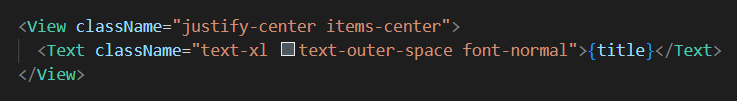
\includegraphics[width=1\textwidth,width=12cm, height=2cm]{images/twrn_styled.png}
	\caption{Tailwind styled View}
	\label{fig:twrn}
\end{figure}
    Styling in the app is primarily achieved using NativeWind which uses tailwind CSS as scripting language to create a universal style system for React Native. NativeWind components can be shared between platforms and will output their styles as CSS StyleSheet on web and StyleSheet.create for native. It provides utility classes that simplify the styling process. However, custom styles are also defined in the styles.js file, which allows for additional customization and flexibility in styling the app's components. \cite{nativewinddocs}

The codebase follows a modular approach, organizing components into separate files for reusability throughout the app. These custom components serve specific purposes and are imported into files using 'import' statements at the top. Additionally, the app utilizes external resources, such as image storage, which are further explained in the API section (refer to Section~\ref{sec:api}) for more details. This modular structure enhances code organization and promotes code reusability, making it easier to maintain and expand the application.\\
Components used in this app are functional components and are reusable, lightweight and use custom styling. To use the component, import from /src/views/components and include it in your desired screens or components. If there are any additional dependencies required, they are mentioned. Most items use styling from tailwind CSS in the component file, otherwise default styles are extended.
\begin{compactenum}
    \item ButtonComponent:
    \begin{itemize}
        \item API Documentation: It accepts props such as title, onPress to customize its appearance and behavior. It is used in Register Screen, Login Screen, Matches Screen etc.
        \item Interactions: It triggers the onPress event when pressed, allowing developers to define the desired functionality. 
    \end{itemize}
    \item TextInputComponent:
    \begin{itemize}
        \item Overview: The TextInputComponent provides an input field for users to enter text.
        \item API Documentation: The TextInputComponent accepts props such as label, icon, error, password and onFocus function to manage the input field's content and appearance.
        \item Dependencies: This component also uses MaterialCommunityIcons from @expo/vector-icons package.
        \item Interactions: This component is used to render input fields on Register and Login Screen. It shows different styling to handle errors such as empty input field errors and also implements password field's secure text entry by enabling user to hide or show password by pressing on an icon. It sets the outlines of the text input boxes as darker or red in case of focus or errors respectively. 
    \end{itemize}
    \item ChatList:
    \begin{itemize}
        \item API Documentation: The ChatList component uses FlatList from react native, user and buddies from Context API (more on Context API in Section~\ref{sec:api}).
        \item Interactions: The ChatList component is the only component other than header that is rendered on Messages screen. It shows list of chats.
    \end{itemize}
    \item ChatRow:
    \begin{itemize}
        \item API Documentation: The ChatRow component accepts props which is data of the buddy with whom the chat is, such as email, name, messageId and photo to display chat information on the messages screen.
        \item Dependencies: It uses useNavigation hook from react-navigation/native to navigate to chat screen.
        \item Interactions: The component triggers the onPress event when clicked to be taken to Chat Screen where the chat of the logged in user with the buddy is displayed.
    \end{itemize}
    \item ReceiverMessage and SenderMessage:
    \begin{itemize}
        \item Overview: The ReceiverMessage and SenderMessage components represent message bubbles for received and sent messages, respectively.
        \item API Documentation: Both components accept props such as message and time, ReceiverMessage component also accepts photourl as prop so it can load the receiver's profile picture with the message bubble.
        \item Interactions: The ReceiverMessage and SenderMessage components do not handle any specific interactions but can be combined with other components for messaging functionality.
    \end{itemize}
    \item CustomDrawerContent:
    \begin{itemize}
        \item Overview: The CustomDrawerContent component provides a customized drawer menu for navigation through drawer navigator. 
        \item API Documentation: Usually it is a self contained component however, it displays logged in user's name, profile picture and buddy count therefore it requires props from drawer navigator which uses context API.
        \item Dependencies: The component uses several packages like react-native-paper for use of Avatar, text styles, sections. It also uses packages like @react-navigation/drawer for building custom drawer by using its scroll view and drawer items list components. Other than that, @expo/vector-icons and @react-navigation/native packages are used for icons and handling navigation respectively.
        \item Interactions: It can be opened on any drawer screens either by tapping the navicon from the header on top left corner or by sliding the screen towards right. One can navigate to Home, Edit Profile, Matches and Contact Us screens or can tap the logout button for logging out of the app.
    \end{itemize}
    \item Header:
    \begin{itemize}
        \item API Documentation: The Header component accepts props such as title to customize its content.
        \item Dependencies: Header also uses icon and navigation from @expo/vector-icons and @react-navigation/native packages.
        \item Interactions: This particular header component is actually used in navigation from messages screen to chat screen to display name of the 'buddy' the user is engaging in messages with.
    \end{itemize}
    \item ImageComponent:
    \begin{itemize}
        \item API Documentation: The ImageComponent only accepts a prop called 'card' to check if users being displayed on home screen have valid profile pictures or not. It displays image if a user has the image otherwise it handles the error by setting the image to a placehold url.
    \end{itemize}
    \item Loader:
    \begin{itemize}
        \item Overview: Loader displays react native's ActivityIndicator and a custom styled loading container with text during data fetching or processing.
        \item API Documentation: The Loader component normally manages its own internal state, but it requires a boolean called visible to make handling its visibility in different API calls, easier.
    \end{itemize}
\end{compactenum}

\subsection{Building}\label{subsec:build}
The tools needed for development are already mentioned in Section~\ref{sec:dev_tools}. Here are mentioned the tools needed to generate APK for fast packaging and distribution.\\
The packaging and building is handled by Expo through EAS (Expo Application Services) which are the cloud services for the React Native Expo apps. EAS Build is a hosted service for building app binaries for Expo and React Native projects. \cite{easdoc}\\
\textbf{Install the EAS CLI}\\
EAS CLI is the dedicated command line for Expo Application Services.
\mint{console}|npm install -g eas-cli|
\textbf{Log in to your Expo account}\\
An Expo account is needed to use Expo Services which offers 30 lower-priority builds (of those, up to 15 iOS) per month with build timeout upto 45 minutes.
\mint{console}|eas login|
\textbf{Create a configuration file}\\
Configure EAS as shown:
\mint{console}|eas build:configure|
Select the platforms for which you would like to configure EAS Build. In this case it will be Android. This will generate an "eas.json" file. Modify the build settings as per needed. For APK, just edit the "preview" option as shown in the snippet~\ref{src:eas}.
\begin{listing}[H]
\begin{minted}{json} 
{
"preview": {
      "android": {
        "buildType": "apk"
      }
    },
}
\end{minted}
\caption{eas.json}
\label{src:eas}
\end{listing}

\textbf{Run a build}\\
Before the build can start, you’ll need to generate or provide app signing credentials. \cite{eascred}
\mint{console}|eas build -p android --profile preview|
\subsection{Persistent Data Storage and State Management}\label{subsec:storage}
In the app, AsyncStorage is used to store items related to the "user" entity. AsyncStorage is a storage system provided by React Native that allows key-value pairs to be persisted locally on the device. By utilizing AsyncStorage, data related to the user can be saved and retrieved across different app sessions.

To simplify the handling of AsyncStorage, a single file is dedicated to the implementation of the Context API present in the api folder as shown by the folder structure in Figure~\ref{fig:codebase}. The Context API allows for the creation and management of global application state. In this case, the main navigator in App.js is wrapped with the UserProvider from the Context API, ensuring that the data stored in the context is accessible throughout the app. This approach eliminates the need for making costly API calls on each screen and helps to optimize performance.

One drawback of the Context API is that it can potentially load all values even if only a specific object is needed. To address this, the useMemo hook and memoized values are utilized within the Context API. By specifying dependencies in the dependency array, only the necessary values are updated when the Context API is called, preventing unnecessary re-rendering and recreating of context values.

By managing all states in the Context API, the need to use useEffect on every screen multiple times is eliminated. Instead, useFocusEffect and useCallback are employed on screens where data needs to be refreshed after specific processes. The useFocusEffect hook ensures that the defined refresh methods are called when the screen comes into focus, while useCallback optimizes the performance of the refresh methods by memoizing their values and preventing unnecessary re-renders.

Most APIs responsible for fetching data from the back-end, login functionality and signout is being handled in context API. On signout function call, several actions are performed to ensure proper cleanup and logout. 
\begin{compactenum}
    \item The "user" item stored in AsyncStorage is removed, effectively clearing the user's data from storage.
    \item All relevant data stored in the state variables is cleared, ensuring that any user-related information is reset.
    \item Additionally, the timer responsible for automatically logging out the user is cleared to prevent any further automatic logout actions from occurring.
\end{compactenum}
These steps collectively ensure that the user's data is securely cleared, state variables are reset, and any automatic logout mechanisms are halted upon sign-out.
Overall, the combination of AsyncStorage, the Context API, memoized values in useMemo, useFocusEffect, and useCallback helps to efficiently manage data, reduce API calls, and optimize performance throughout the app.
\newline
For backend data storage, the app utilizes Firestore, a real-time NoSQL database. Firestore maintains collections of documents, and in this app, two main documents are used: "user" and "messages". The "user" document contains a collection of user profiles, while the "messages" document stores a map of messages exchanged between users.

To ensure data security, most API calls in the app are POST requests that include a token specific to the logged-in user. This token is then verified using Firebase JWT tokens, which helps authenticate and authorize the user on the back-end, thereby ensuring app security.

A more detailed description of the database structure and functionality can be found in the appendix~\ref{appx:backend_doc} dedicated to back-end and database structure.
\subsection{Backend and Third-Party Services}
The application utilizes a Node.js backend with Firebase integration. The backend is responsible for handling various functionalities of the app, including user authentication and data management. Additionally, images are uploaded to the app through a third-party application called Cloudinary.

The backend of the application is hosted on OnRender, providing a reliable hosting environment for the server-side components. The database used for storing app data is Firestore, Firebase's NoSQL database, which offers flexibility and scalability for managing and organizing data.

There are several reasons for incorporating a backend with Firebase in the Study Buddy app. Firstly, the mobile app is controlled and managed through an admin web application developed using Flask. This allows for efficient administration and monitoring of the app's operations.

Additionally, the backend implementation includes the AI integration in the form of a recommendation algorithm model using OpenAI API. This algorithm enhances the app's functionality by providing personalized study partner recommendations to users based on their preferences.

To ensure secure user authentication, Firebase JWT authentication is implemented in the app. This means that token validation is performed through the backend, providing an extra layer of security by validating user access through the backend server rather than directly accessing Firestore documents.

These backend components and integration contribute to the overall functionality and user experience of the Study Buddy app, enabling seamless communication, personalized recommendations, and secure user authentication. More on this is mentioned in the documentation dedicated to back-end and storage.
\section{API Documentation}\label{sec:api}
This section provides an overview of the API calls used on the client-side to retrieve and submit data. The endpoints described here have been thoroughly tested by the backend developer using Postman (more detailed description see appendix~\ref{appx:backend_doc}), ensuring their reliability and functionality. By following the instructions and examples provided, you will be able to effectively make API calls from the client-side of your application to the server hosted on Render hosting service.
\subsection{Registration}
\begin{table}[H]
	\centering
	\begin{tabular}{ |p{0.3\textwidth}|p{0.3\textwidth}|p{0.3\textwidth}| }
		\hline
            \multicolumn{3}{|c|}{/createUser} \\
            \hline
		\textbf{Method} & \textbf{Parameters} & \textbf{Location}\\
            \hline
		  POST & name, email, password & RegisterScreen.js\\
            \hline
	\end{tabular}
	\caption{API Description for Registration}
	\label{tab:signup}
\end{table}
The API is being called to register user to the hosted server. The call is posting data stored in 'inputs' object state as shown in the code snippet~\ref{src:register}. 
\begin{listing}[H]
\begin{minted}{js} 
  const signUpFunction = async () => {
    const url = "https://studybuddy-backend.onrender.com/createUser";
    setLoading(true);
    setTimeout(async () => {
      setLoading(false);
      try {
        const response = await axios.post(url, inputs);
        if (response.status === 200) {
          try {
            await AsyncStorage.setItem("user", JSON.stringify(inputs));
            navigation.navigate("Login");
          } catch (error) {
            Alert.alert("Error", "Something went wrong with app's storage.");
          }
        } else {
          Alert.alert("Error", "Something went wrong");
        }
      } catch (e) {
        Alert.alert("Error", "Email already exists, choose a different email.");
      }
    }, 3000);
  };
\end{minted}
\caption{Client-side API Call}
\label{src:register}
\end{listing}

% @@@@@@@@@@@@@@@@@@@@@@@@@@@22
\subsection{Login}
\begin{table}[H]
	\centering
	\begin{tabular}{ |p{0.3\textwidth}|p{0.3\textwidth}|p{0.3\textwidth}| }
		\hline
            \multicolumn{3}{|c|}{/signIn} \\
            \hline
		\textbf{Method} & \textbf{Parameters} & \textbf{Location}\\
            \hline
		  POST & email, password & UserContext.js\\
            \hline
	\end{tabular}
	\caption{API Description for Login}
	\label{tab:login}
\end{table}
The API is being called to login user by posting user information~\ref{src:login}. As seen from \ref{tab:login} that the function is located inside Context API and is being called on the login screen by using useContext() from React. This is how user is available to the entire app with UserContext Provider acting as a wrapper, and hence making it easier to handle routing as explained in section~\ref{subsec:storage}. This function also handles whether the user has completed profile or not by using 'flag'.
\begin{listing}[H]
\begin{minted}{js} 
  const loginFunction = async (email, password, navigation) => {
    const url = "https://studybuddy-backend.onrender.com/signIn";
    try {
      const response = await axios.post(url, {
        email: email,
        password: password,
      });
      if (response.status === 200) {
        if (response?.data?.token) {
          setToken(response?.data?.token);
          const flag = response?.data?.flag;
          let userData = {
            token: response?.data?.token,
            email: email,
            flag: flag,
          };
          if (flag) {
            AsyncStorage.setItem(
              "user",
              JSON.stringify({ ...userData, loggedIn: true })
            );
            setIsLoggedIn(true);
            navigation.navigate("Drawer");
          } else {
            AsyncStorage.setItem(
              "user",
              JSON.stringify({ ...userData, loggedIn: false })
            );
            navigation.navigate("CompleteProfile");
          }
        } else {
          Alert.alert("Error", "Invalid Login!");
        }
      } else {
        setLoading(false);
        Alert.alert("Request failed", "Something went wrong!");
      }
    } 
  };
\end{minted}
\caption{Client-side API Call}
\label{src:login}
\end{listing}
% @@@@@@@@@@@@@@@@@@@@@@@@@@@22
\subsection{Complete Profile}\label{subsec:complete_profile}
\begin{table}[H]
	\centering
	\begin{tabular}{ |p{0.3\textwidth}|p{0.3\textwidth}|p{0.3\textwidth}| }
		\hline
            \multicolumn{3}{|c|}{/setUserData , image upload} \\
            \hline
		\textbf{Method} & \textbf{Parameters} & \textbf{Location}\\
            \hline
		  POST & token, name, age, Language, Major, InterestedSubjects, Location, University, bio, photoUrl, flag & CompleteProfile.js\\
            \hline
		  POST & uri, photo name, photo type & CompleteProfile.js\\
            \hline
	\end{tabular}
	\caption{API calls on Complete Profile Screen}
	\label{tab:complete_profile}
\end{table}
The setUserData is being called to post user data to the server. This API is also used on Edit Profile page.
\begin{listing}[H]
\begin{minted}{js} 
  const setUserData = async () => {
    const url = "https://studybuddy-backend.onrender.com/setUserData";
    try {
      const postData = {
        token: token,
        name: inputs.account_name,
        age: age,
        Language: selectedLanguages,
        Major: selectedMajor,
        InterestedSubjects: selectedCourses,
        Location: selectedLocation,
        University: selectedUniversity,
        bio: inputs.bio,
        photoUrl: uploadedImageUrl || image,
        flag: true,
      };
      const response = await axios.post(url, postData);
      if (response.status === 200) {
        setUploadedImageUrl("");
        setImage("");
        setTimeout(() => {
          navigation.navigate("Drawer");
        }, 3000);
      } else {
        Alert.alert("Request Failed!", "Something went wrong!");
      }
    } catch (e) {
      Alert.alert("Error", "Something went wrong!");
    }
  };
\end{minted}
\caption{Client-side API Call for setting user data}
\label{src:complete_profile}
\end{listing}
The is the API call made to Cloudinary (see section~\ref{sec:libraries}) in case user uploads a profile picture. The response then generates a url that can be sent to server to store as user's photoUrl.
\begin{listing}[H]
\begin{minted}{js} 
  const handleUpload = async (image) => {
    const data = new FormData();
    let uriParts = image.split(".");
    let fileType = uriParts[uriParts.length - 1];
    data.append("file", {
      uri: image,
      name: `photo.${fileType}`,
      type: `image/${fileType}`,
    });
    data.append("upload_preset", "study_buddy");
    const url = "https://api.cloudinary.com/v1_1/dg8969jxs/image/upload";
    const config = {
      headers: {
        "Content-Type": "multipart/form-data",
      },
    };
    try {
      setLoading(true);
      const response = await axios.post(url, data, config);
      setUploadedImageUrl(response.data.secure_url);
      setLoading(false);
    } catch (error) {
      setLoading(false);
      if (error.response) {
        console.log(error.response.data);
        console.log(error.response.status);
        console.log(error.response.headers);
      } else if (error.request) {
        console.log(error.request);
      } else {
        Alert.alert(
          "Error",
          "Something happened in setting up the request that triggered an Error"
        );
      }
      console.log(error.config);
      Alert.alert(
        "Error",
        "Something happened in setting up the request that triggered an Error"
      );
    }
  };
\end{minted}
\caption{API call to Cloudinary (Image Upload)}
\label{src:getallotherusers}
\end{listing}
% @@@@@@@@@@@@@@@@@@@@@@@@@@@@@@
\subsection{Home}
\begin{table}[H]
	\centering
	\begin{tabular}{ |p{0.3\textwidth}|p{0.3\textwidth}|p{0.3\textwidth}| }
		\hline
            \multicolumn{3}{|c|}{/getAllOtherUsers , /swipe} \\
            \hline
		\textbf{Method} & \textbf{Parameters} & \textbf{Location}\\
            \hline
		  GET & token (Bearer) & UserContext.js\\
            \hline
		  POST & email, buddy\_email, swipe & UserContext.js\\
            \hline
	\end{tabular}
	\caption{API calls on home screen}
	\label{tab:getallotherusers}
\end{table}
The first API is being called to fetch all the other authenticated users that are not the currently logged in user or their buddies. This way user can still swipe on them.
\begin{listing}[H]
\begin{minted}{js} 
  const fetchAllOtherUsers = async (token) => {
    if (!user || !token) return;
    setLoading(true);
    try {
      const url = 
      "https://studybuddy-backend.onrender.com/getAllOtherUsers";
      axios
        .get(url, { headers: { Authorization: `Bearer ${token}` } })
        .then((res) => {
          if (res.data) {
            setAllOtherUsers(res.data);
            setSwipedData(res.data[0]);
            setLoading(false);
          } else {
            Alert.alert("Error", "An error occurred, please try again later.");
            setLoading(false);
          }
        });
    } catch (error) {
      setLoading(false);
      Alert.alert("Error", "An error occurred, please try again later.");
    }
  };
\end{minted}
\caption{Client-side API Call for getting users}
\label{src:getallotherusers}
\end{listing}
The /swipe API posts the swipe information to the server to handle users' connections. Here the navigation to "MatchModal" also mimics the effect of a notification.
\begin{listing}[H]
\begin{minted}{js} 
  const swipe = async (direction, navigation) => {
    const url = "https://studybuddy-backend.onrender.com/swipe";
    try {
      const response = await axios.post(url, {
        email: user.email,
        buddy_email: swipedData?.email,
        swipe: direction,
      });
      if (response.status === 200) {
        refreshBuddies(); // refresh buddies if swipe happens
        if (response.data.isMatch && direction === true) {
          navigation.navigate("MatchModal", {
            newBuddy: swipedData,
            loggedInUser: user,
          });
        }
      }
    } catch (e) {
      Alert.alert("Error " + e.message);
    }
  };
\end{minted}
\caption{Client-side API Call for Swipe}
\label{src:getallotherusers}
\end{listing}
% @@@@@@@@@@@@@@@@@@@@@@@@@@@@@@
\subsection{Matches}
\begin{table}[H]
	\centering
	\begin{tabular}{ |p{0.3\textwidth}|p{0.3\textwidth}|p{0.3\textwidth}| }
		\hline
            \multicolumn{3}{|c|}{/getBuddies, /getUserData/:uid, /removeBuddy} \\
            \hline
		\textbf{Method} & \textbf{Parameters} & \textbf{Location}\\
            \hline
            POST & token (Bearer) & UserContext.js\\
            \hline
		  GET & - & UserContext.js\\
            \hline
		  POST & token, buddy\_email, swipe & Matches.js\\
            \hline
	\end{tabular}
	\caption{API calls on home screen}
	\label{tab:matches}
\end{table}
The getBuddies api does two jobs of getting all buddies and then being able to select one from all based on uid.
\begin{listing}[H]
\begin{minted}{js} 
const fetchBuddies = async (token) => {
  try {
    const response = await axios.post(
    "https://studybuddy-backend.onrender.com/getBuddies",{token: token,});
      if (response.status === 200) {
      const url = 
    `https://studybuddy-backend.onrender.com/getUserData/${buddyId}`
        const buddyData = await Promise.all(
        response.data.map(async (buddyId) => {
            const buddyResponse = await axios.get(url);
            return buddyResponse.data;
        })
        );
        setBuddies(buddyData);
    } else {
        Alert.alert("Error", "An error occurred, 
        please try again later.");
    }
} catch (error) {
    Alert.alert("Error", "An error occurred, please try again later.");
    }
};
\end{minted}
\caption{Client-side API Call for getting buddies}
\label{src:buddies}
\end{listing}
The /removeBuddy API call deletes the buddy.
\begin{listing}[H]
\begin{minted}{js} 
const removeBuddy = async (token, buddy_email) => {
    try {
      const response = await axios.post(
    "https://studybuddy-backend.onrender.com/removeBuddy",
        {
          token: token,
          buddy_email: buddy_email,
        }
      );
      if (response.status === 200) {
        refreshBuddies();
      } else {
        Alert.alert("Error", "Something went wrong");
      }
    } catch (err) {
      Alert.alert("Error", "Something went wrong");
    }
  };
\end{minted}
\caption{Client-side API Call for Deleting Buddy}
\label{src:buddies-remove}
\end{listing}
% @@@@@@@@@@@@@@@@@@@@@@@@@@@@@@
\subsection{Messaging}
\begin{table}[H]
	\centering
	\begin{tabular}{ |p{0.3\textwidth}|p{0.3\textwidth}|p{0.3\textwidth}| }
		\hline
            \multicolumn{3}{|c|}{/sendMessage, /getMessages2} \\
            \hline
		\textbf{Method} & \textbf{Parameters} & \textbf{Location}\\
            \hline
		  POST & token, buddy\_email, message & ChatScreen.js\\
            \hline
		  POST & messageID & ChatScreen.js\\
            \hline
	\end{tabular}
	\caption{API calls on chat screen}
	\label{tab:chat}
\end{table}
The send message sets input to empty afterwards and also gets message as its not real-time messaging.
\begin{listing}[H]
\begin{minted}{js} 
const sendMessage = async () => {
    const url = "https://studybuddy-backend.onrender.com/sendMessage";
    try {
      const postData = {
        token: token,
        buddy_email: email,
        message: input,
      };
      const response = await axios.post(url, postData);
      if (response.status === 200) {
        setInput("");
        getMessages();
      } else {
        Alert.alert("Error", "Something went wrong!");
      }
    } catch (e) {
      Alert.alert("Error", "Something went wrong!");
    }
  };
\end{minted}
\caption{Client-side API Call for sending messages}
\label{src:chat-send}
\end{listing}
The API call for get message only happens when the screen is mounted or when user sends a message.
\begin{listing}[H]
\begin{minted}{js} 
const getMessages = async () => {
    const url = "https://studybuddy-backend.onrender.com/getMessages2";
    try {
      const postData = {
        chatId: messageDetails,
      };
      const response = await axios.post(url, postData);
      if (response.status === 200) {
        const sortedMessages = response.data.sort((a, b) => {
          return new Date(b.time) - new Date(a.time);
        });
        setMessages(sortedMessages);
        await refreshUser();
      } else {
        Alert.alert("Error", "Something went wrong!");
      }
    } catch (e) {
      Alert.alert("Error", "Something went wrong!");
    }
  };
\end{minted}
\caption{Client-side API Call for Getting Messages}
\label{src:chat-get}
\end{listing}
% @@@@@@@@@@@@@@@@@@@@@@@@@@@@@@
\subsection{Delete Account}
\begin{table}[H]
	\centering
	\begin{tabular}{ |p{0.3\textwidth}|p{0.3\textwidth}|p{0.3\textwidth}| }
		\hline
            \multicolumn{3}{|c|}{/deleteProfile} \\
            \hline
		\textbf{Method} & \textbf{Parameters} & \textbf{Location}\\
            \hline
		  POST & token (Bearer) & MyProfile.js\\
            \hline
	\end{tabular}
	\caption{API Description for Deleting Account}
	\label{tab:delete}
\end{table}
The API is being called on Edit Profile page and deletes user's account and redirects user to Login Page.
\begin{listing}[H]
\begin{minted}{js} 
const deleteAccount = async () => {
    const url = "https://studybuddy-backend.onrender.com/deleteProfile";
    try {
      const postData = {
        token: token,
      };
      const response = await axios.post(url, postData);
      if (response.status === 200) {
        signOut(false);
        Alert.alert("Success", "Your account was deleted!");
      } else {
        Alert.alert("Request Failed", "Something went wrong, try again later!");
      }
    } catch (e) {
      Alert.alert("Error", "Something went wrong!");
    }
  };
\end{minted}
\caption{Client-side API Call}
\label{src:delete}
\end{listing}
% @@@@@@@@@@@@@@@@@@@@@@@@@@@22
\section{Architecture}\label{sec:nav_map}
The navigational directions based on the app's architecture given by material design\cite{navtypes} are as follows:
\begin{compactitem}
    \item \textbf{Lateral Navigation:} The primary navigation component of the app, the Drawer Navigator, provides access to all top-level destinations. Users can seamlessly switch between screens such as Home, My Profile, Matches, and Contact Us, allowing them to explore different sections of the app without losing context.
    \item \textbf{Forward Navigation:} Forward navigation involves moving between screens at consecutive levels of hierarchy or steps in a flow. Users can navigate forward by interacting with various components, such as buttons or links, to access different sections of the app. For example, on the Home screen, users can swipe cards right or left using the React Native Deck Swiper component, which opens the User Info Modal screen for each card, providing detailed information about the user. Similarly, on the Matches screen, users can open the Buddy Info Modal to view additional details about a specific match. This forward navigation functionality in Study Buddy ensures smooth transitions and empowers users to explore and engage with the app's features effortlessly.
    \item \textbf{Reverse Navigation:} Reverse navigation allows users to move backward through screens either chronologically or hierarchically. Chronological reverse navigation refers to moving backward through the app's screens in the order in which they were accessed. For instance, users can go back from the Chat screen to the Messages screen to revisit their conversations. Hierarchical reverse navigation follows platform conventions and allows users to navigate back within the app's navigation hierarchy. Users can, for example, return from the My Profile screen to the Home screen by using the back button or react native gesture handler.
    By incorporating lateral, forward, and reverse navigation within the StudyBuddy app, users can easily explore and interact with different screens, smoothly progress through different levels of hierarchy, and effortlessly navigate backward to revisit previous screens or steps in their user journey.
\end{compactitem}
\subsection{Navigational Hierarchy}\label{subsec:nav_hierarchy}
The navigational hierarchy demonstrates the structure of the app's screens and how they are organized within the Navigation Container and Stack.Navigator. The Stack.Navigator manages the screens and their navigation options within the app.
Based on the isLoggedIn state, the Stack.Navigator renders different screen groups. When isLoggedIn is true, the app renders screens related to the authenticated user. These screens include a Drawer.Navigator, which serves as the main navigation for the app. It contains screens such as HomeScreen, MyProfile, Matches, and ContactUs. Additionally, there are screens like MessagesScreen and ChatScreen for managing messages and conversations between users. The app also includes modal screens, UserInfoModal and BuddyInfoModal, for displaying user information. Another modal screen, MatchModal, is used to show matching results.
When isLoggedIn is false, indicating that the user is not authenticated, the app renders screens for the user authentication process. These screens include GetStartedScreen, OnboardingSlider, RegisterScreen, LoginScreen, and CompleteProfile.\newline
The application's navigational hierarchy consists of a NavigationContainer component which holds one Stack Navigator only which holds different screens. The hierarchy is as follows:
        \begin{itemize}
            \item Stack.Group (isLoggedIn)
            \begin{itemize}
                \item Stack.Screen (name: "Drawer", component: DrawerNavigator)
                \begin{itemize}
                    \item Drawer.Navigator
                    \begin{itemize}
                        \item Drawer.Screen (name: "Home", component: HomeScreen)
                        \item Drawer.Screen (name: "MyProfile", component: MyProfile)
                        \item Drawer.Screen (name: "Matches", component: Matches)
                        \item Drawer.Screen (name: "ContactUs", component: ContactUs)         
                    \end{itemize}
                \end{itemize}
                \item Stack.Screen (name: "Messages", component: MessagesScreen)
                \item Stack.Screen (name: "Chat", component: ChatScreen)
                \item Stack.Group (Modal Screens)
                \begin{itemize}
                    \item Stack.Screen (name: "UserInfoModal", component: UserInfoModal)
                    \item Stack.Screen (name: "BuddyInfoModal", component: BuddyInfoModal)
                \end{itemize}
                \item Stack.Group (transparent Modal Screen)
                \begin{itemize}
                    \item Stack.Screen (name: "MatchModal", component: MatchModal)
                \end{itemize}
            \end{itemize}
            \item Stack.Group (!isLoggedIn)
            \begin{itemize}
                \item Stack.Screen (name: "GetStarted", component: GetStartedScreen)
                \item Stack.Screen (name: "OnboardingSlider", component: OnboardingSlider)
                \item Stack.Screen (name: "Register", component: RegisterScreen)
                \item Stack.Screen (name: "Login", component: LoginScreen)
                \item Stack.Screen (name: "CompleteProfile", component: CompleteProfile)
            \end{itemize}
        \end{itemize}
\subsection{Navigation Map}
\begin{figure}[H]
	\centering
	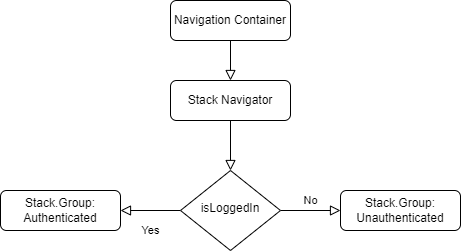
\includegraphics[width=1\textwidth,width=10cm, height=6cm]{images/SB_nav_container.png}
	\caption{Navigation Map}
	\label{fig:navmap}
\end{figure}
Based on the hierarchy represented in the subsection \ref{subsec:nav_hierarchy}, we have constructed a navigation map in  Figure~\ref{fig:navmap} which provides a visual representation of the navigational flow of the app's screens. It showcases the conditional rendering based on the isLoggedIn state, highlighting the screens available to authenticated and unauthenticated users shown in Figure~\ref{fig:navmap_auth} and Figure~\ref{fig:navmap_unauth} respectively.
\begin{figure}[H]
	\centering
	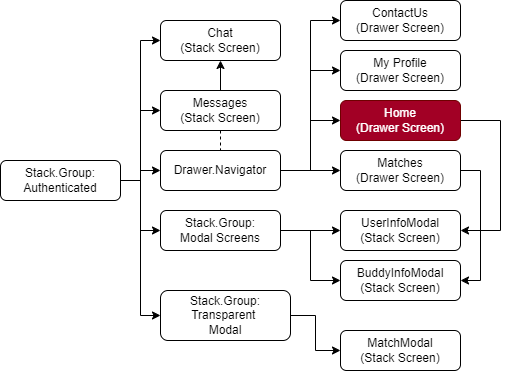
\includegraphics[width=1\textwidth,width=15cm, height=10cm]{images/SB_auth.png}
	\caption{Navigation Map (if user is logged in)}
	\label{fig:navmap_auth}
\end{figure}
In case where isLoggedIn state is set to \emph{true} the initial route is set to Home Screen as shown in Figure~\ref{fig:navmap_auth}. The Messages screen is available through header section of the app from Drawer Screens. The diagram shows the inclusion in Stack if user is autheticated. For instance, authenticated user can only reach to Chat screen through Messages screen but Chat is still a part of the given stack group. The user flow of the app will be shown in Section~\ref{sec:user_flow}.
\begin{figure}[H]
	\centering
	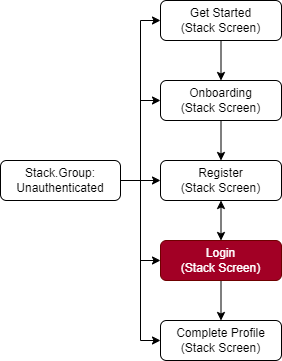
\includegraphics[width=1\textwidth,width=8cm, height=8cm]{images/SB_unauth.png}
	\caption{Navigation Map (if user is not logged in)}
	\label{fig:navmap_unauth}
\end{figure}
Similarly, in the case where isLoggedIn state is set to \emph{false} the initial route is set to Login Screen as shown in Figure~\ref{fig:navmap_unauth}. The user can switch between Registration and Login screens. In order to navigate to authenticated stack, user needs to complete profile from Complete Profile screen.
\section{Libraries and Sources}\label{sec:libraries}
The application utilizes various third-party libraries and services to enhance frontend design and streamline development. Notable libraries include expo/vector-icons and expo-image for creating an appealing frontend design. The decision to incorporate expo-image was made during the later stages of development due to caching issues discovered during testing, which will be discussed further in Section~\ref{subsec:testing-findings}.
Additionally, the following external sources were utilized:
\begin{compactitem}
    \item \textbf{Figma:} Used for creating icons, splash screens, and wireframes.
    \item \textbf{Expo Metro Bundler:} Employed as a reliable bundling tool within the Expo ecosystem. (Used by Expo-CLI) \cite{MetroDoc}
    \item \textbf{Coolors:} Utilized to generate a color palette for the application's design. \cite{coolors}
    \item \textbf{Tailwind CSS:} Adopted for simplified styling capabilities. \cite{tailwind}
    \item \textbf{Cloudinary:} Integrated as an image storage service. \cite{cloudinary}
    \item \textbf{Alphabetical Sorter:} VS code extention used in sorting JSON data used in dropdowns.
    \item \textbf{Icon-Library:} Leveraged as a free icon library to generate logos, icons, and images for various screens, including the app icon. \cite{icon-library}
    \item \textbf{gifgit.com:} Provided free online tools for editing the said icons and images.
    \item \textbf{OpenAI API:} Users can conveniently check their recommendation scores by accessing the admin web app of our mobile application. More on this is detailed in section~\ref{subsec:recommendations}.
\end{compactitem}
These third-party resources were instrumental in achieving the desired functionality and aesthetics of the application.
\section{Testing Plan}\label{sec:testing-plan}
In the case of testing frontend, mostly unit testing is implemented with jest version 29.2.1 and jest-expo 48.02.2. The entire user-flow is tested by end-to-end (e2e) testing. The unit testing with jest is both white box and black box in this case, here is how:
\begin{compactenum}
    \item White Box Testing:
    \begin{compactitem}
        \item The test cases will access the internal implementation details of components. They render the component using render() from the @testing-library/react-native package and make assertions based on the component's internal state or properties.
        \item Example would be testing the presence of specific elements or properties like getByTestId, getByText, and accessing props.style.opacity as shown in the following code snippet~\ref{src:buttoncomponent} \newline

\begin{listing}[H]
\begin{minted}{js} 
import React from "react";
import { fireEvent, render } from "@testing-library/react-native";
import ButtonComponent from "../../../../src/views/components/ButtonComponent";

describe("Button Component", () => {
  afterEach(() => {
    jest.clearAllMocks();
  });

  test("1. Render Button", () => {
    const { getByTestId } = render(<ButtonComponent title="Test Title" />);
    expect(getByTestId("button")).toBeTruthy();
  });

  test("2. Title and disabled props", () => {
    const { getByText, getByTestId } = render(<ButtonComponent title="Test Title" disabled={true} />);
    expect(getByText("Test Title")).toBeTruthy();
    expect(getByTestId('pressButton').props.style.opacity)
    .toBe(0.3);
  });

  test("3. Button onPress function", () => {
    const mockOnPress = jest.fn();
    const { getByTestId } = render(<ButtonComponent title="Test Title" onPress={mockOnPress} />);
    
    fireEvent.press(getByTestId('pressButton'));
    expect(mockOnPress).toHaveBeenCalledTimes(1);
  });
});
\end{minted}
\caption{Testing ButtonComponent}
\label{src:buttoncomponent}
\end{listing}
    \end{compactitem}
    \item Black Box Testing:
    \begin{compactitem}
        \item The test cases also focus on the external behavior of the components. They interact with the rendered component as a black box without considering the internal implementation details.
        \item Examples of black box testing in the app are simulating button presses using fireEvent.press and checking the expected behavior or side effects, such as verifying that the mockOnPress function is called as shown in the code snippet~\ref{src:buttoncomponent}.
        
    \end{compactitem}
\end{compactenum}
\section{Testing Execution}\label{sec:testing-execution}
\subsection{Unit Testing}
For unit testing with Jest, tests are written using the Jest testing syntax and can be organized into test suites and test cases. For testing its the same working tree as that of the src directory but in tests folder. Tests are typically placed in separate files within the test directory, following a naming convention (e.g. '*test.js'). \\
\textbf{Mocking Dependencies:} Jest allows for easy mocking of dependencies, such as API calls or external libraries, to isolate and control the behavior of the code being tested. Mocking is useful for focusing on specific code paths, simulating different scenarios, and avoiding unwanted side effects during testing. This mocking is mainly done in the mocks folder as shown in Figure~\ref{fig:codebase_test}.

\begin{figure}[H]
	\centering
	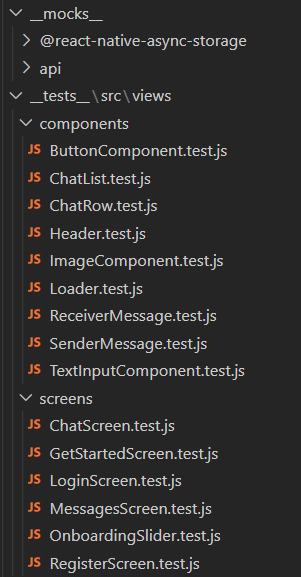
\includegraphics[width=1\textwidth,width=6cm, height=12cm]{images/testing_code_tree.png}
	\caption{Folder Structure (Tests)}
	\label{fig:codebase_test}
\end{figure}

All the major code components are tested with unit testing by Jest. There are 15 test suites and 32 test cases as shown in figure~\ref{fig:passed_Tests}.

\begin{figure}[H]
	\centering
	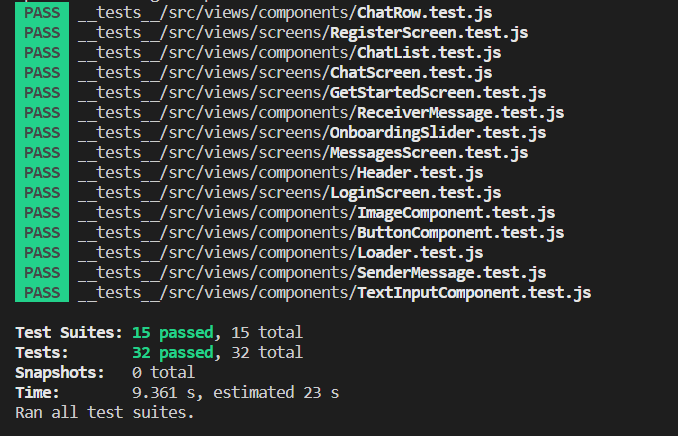
\includegraphics[width=1\textwidth,width=14cm, height=10cm]{images/test_passing.png}
	\caption{Passed Test Cases}
	\label{fig:passed_Tests}
\end{figure}

\subsection{Manual Testing}
The following user stories outline the end-to-end (e2e) testing of the user-flow within the application. These user stories cover various scenarios and interactions that users may encounter while navigating through the app. Each user story represents a specific task or action that a user would perform, allowing us to test the functionality and user experience of the app across different screens and features.
The user stories are presented in a simplified format, using the "Given," "When," "Then," and "And" statements to describe the desired behavior and outcomes of each scenario. 
\\
\textbf{Title: Onboarding Introduction} \\
Scenario:
\begin{compactitem}
    \item Given that I am a new user
    \item When I launch the app for the first time
    \item Then I expect to see an introduction screen with the app-icon, tagline and an option to get started.
\end{compactitem}

\bigskip
\textbf{Title: Navigating to Onboarding Slider} \\
Scenario:
\begin{compactitem}
    \item Given that I have opened the app and I am on the get started screen
    \item When I tap on the "Get Started" button
    \item Then I expect to be navigated to the onboarding slider screen.
\end{compactitem}

\bigskip
\textbf{Title: Viewing Onboarding Slides} \\
Scenario:
\begin{compactitem}
    \item Given that I am on the onboarding slider screen
    \item When I swipe or tap 'Next' to proceed through the slides
    \item Then I expect to see informative slides that showcase the app's key features and benefits.
\end{compactitem}

\bigskip
\textbf{Title: Skipping Onboarding} \\
Scenario:
\begin{compactitem}
    \item Given that I am on the onboarding slider screen
    \item When I choose to skip the onboarding process by tapping 'Skip'
    \item Then I expect to be directed to the last slider screen which shows the 'Register' button.
\end{compactitem}

\bigskip
\textbf{Title: Registering with Full Name, Email, and Password} \\
Scenario:
\begin{compactitem}
    \item Given that I am on the registration screen
    \item When I enter my full name, email, and password
    \item And I tap on the "Register" button
    \item Then I expect my registration information to be validated and stored securely.
    \item And I should be redirected to the login screen.
\end{compactitem}

\bigskip
\textbf{Title: Logging In with Email and Password} \\
Scenario:
\begin{compactitem}
    \item Given that I am on the login screen
    \item When I enter my registered email and password
    \item And I tap on the "Login" button
    \item Then I expect my login credentials to be authenticated.
    \item And I should be directed to the complete profile screen.
\end{compactitem}

\bigskip
\textbf{Title: Navigating to Login or Registration from Registration Screen} \\
Scenario:
\begin{compactitem}
    \item Given that I am on the registration screen
    \item When I view the options below the registration button
    \item Then I expect to see a text prompting me to navigate to the login screen if I already have an account.
\end{compactitem}

\bigskip
\textbf{Title: Navigating to Login or Registration from Login Screen} \\
Scenario:
\begin{compactitem}
    \item Given that I am on the login screen
    \item When I enter my registered email and password
    \item And I tap on the "Login" button
    \item Then I expect my login credentials to be authenticated.
    \item And I should be directed to the complete profile screen.
\end{compactitem}

\bigskip
\textbf{Title: Logging In with Email and Password} \\
Scenario:
\begin{compactitem}
    \item Given that I am on the login screen
    \item When I view the options below the login button
    \item Then I expect to see a text prompting me to navigate to the registration screen if I don't have an account.
\end{compactitem}

\bigskip
\textbf{Title: Skip Completing Profile on Login} \\
Scenario:
\begin{compactitem}
    \item Given that I already have an account
    \item When I log in with my credentials
    \item Then I should be directed straight to the home screen, bypassing the profile completion process.
\end{compactitem}

\bigskip
\textbf{Title: Providing Mandatory Information on Complete Profile} \\
Scenario:
\begin{compactitem}
    \item Given that I have successfully logged in and directed to the complete profile screen
    \item When I enter my account name and select up to four preferred languages from the dropdown menu
    \item And I click on "Next" to proceed to the next step
    \item Then I should be able to navigate back to the previous step by clicking "Previous."
\end{compactitem}

\bigskip
\textbf{Title: Choosing to Finish Profile Later} \\
Scenario:
\begin{compactitem}
    \item Given that I am on the complete profile screen
    \item When I decide to press the "Finish Later" button
    \item Then I should be prompted with an alert message informing me that all entered information will be lost if I proceed.
    \item If I confirm the prompt, I should be taken back to the login screen.
    \item If I cancel the prompt, I should remain on the complete profile screen to continue entering the information.
\end{compactitem}

\bigskip
\textbf{Title: Submitting Complete Profile Information} \\
Scenario:
\begin{compactitem}
    \item Given that I have completed all progress steps of the profile completion process
    \item When I reach the final step and review my information
    \item And I click on the "Submit" button
    \item Then I expect my profile details to be saved
    \item And I should be directed to the home screen to access the full app experience.
\end{compactitem}

\bigskip
\textbf{Title: View on Home Screen} \\
Scenario:
\begin{compactitem}
    \item Given that I am on the home screen
    \item When I access the main screen
    \item Then I should be able to see a swiper component that displays user profile cards. Each card should contain the user's profile picture, name, university, and major information. At the bottom of the screen, there should be two buttons for "Like" and "Dislike" actions. Between the like and dislike buttons, there should be an up arrow button that, when clicked, opens a modal screen displaying additional information about the user.
\end{compactitem}

\bigskip
\textbf{Title: Like and Dislike Buttons with Card Swipe Actions} \\
Scenario:
\begin{compactitem}
    \item Given that I am on the home screen
    \item When I click the "Like" button or perform a swipe right gesture on a user's profile card
    \item Then the user's profile card should be swiped to the right, indicating a positive interaction
\end{compactitem}

\bigskip
\textbf{Title: Notification of Mutual Swipe Right and Buddies Connection} \\
Scenario:
\begin{compactitem}
    \item Given that I have swiped right on a user's profile card on the home screen
    \item When the user I swiped right on also swipes right on my profile card
    \item Then I should receive a transparent modal notification stating this user is now my StudyBuddy with a button to message the new buddy and initiate a conversation.
\end{compactitem}

\bigskip
\textbf{Title: Dislike Button with Card Swipe Action} \\
Scenario:
\begin{compactitem}
    \item Given that I am on the home screen with user profile cards and like/dislike buttons
    \item When I click the "Dislike" button or perform a swipe left gesture on a user's profile card
    \item Then the user's profile card should be swiped to the left, indicating a negative interaction and no notification or action is triggered if the user I disliked swipes left or dislikes my profile card.
\end{compactitem}

\bigskip
\textbf{Title: Modal Screen with User Information on Arrow Button Press} \\
Scenario:
\begin{compactitem}
    \item Given that I am on the home screen with user profile cards and an arrow button at the bottom center
    \item When I tap the arrow button
    \item Then a modal screen should appear, displaying detailed information about the current user on the profile card
\end{compactitem}

\bigskip
\textbf{Title: Navigating to Messages and Sending/Receiving Messages} \\
Scenario:
\begin{compactitem}
    \item Given that I am on the home screen
    \item When I tap on the messages icon in the top-right corner of the screen
    \item Then I should be navigated to the messages screen, where I can view my conversations and select a user to message.
\end{compactitem}

\bigskip
\textbf{Title: Selecting a User to Message} \\
Scenario:
\begin{compactitem}
    \item Given that I am on the messages screen
    \item When I choose a user from the list of conversations
    \item Then I should be directed to a chat interface where I can send and receive messages with that user.
\end{compactitem}

\bigskip
\textbf{Title: Sending and Receiving Messages} \\
Scenario:
\begin{compactitem}
    \item Given that I am in a chat interface with another user
    \item When I type a message and press the send button
    \item Then my message should be sent to the other user, and I should see it in the chat.
    \item If the other user sends a message, I should receive it through an asynchronous API call. To view the received message, I need to navigate back to the messages screen or send another message. 
\end{compactitem}

\bigskip
\textbf{Title: Testing Edit Profile Screen and Account Deletion} \\
Scenario:
\begin{compactitem}
    \item Given that I am on the home screen and have access to the side drawer
    \item When I select the "Edit Profile" option from the side drawer
    \item Then I should be navigated to the edit profile screen.
\end{compactitem}

\bigskip
\textbf{Title: Editing Profile Details on Edit Profile Screen} \\
Scenario:
\begin{compactitem}
    \item Given that I am on the edit profile screen
    \item When I make changes to my profile, such as editing or removing my profile picture, updating personal information, or modifying any other editable fields
    \item And I have filled out all mandatory fields
    \item Then I need to click the "Update Profile" button to save the changes.
\end{compactitem}

\bigskip
\textbf{Title: Deleting My Account on Edit Profile Screen} \\
Scenario:
\begin{compactitem}
    \item Given that I am on the edit profile screen
    \item When I choose the option to delete my account
    \item And I confirm the account deletion
    \item Then I should be taken to the login screen, indicating that my account has been successfully deleted.
\end{compactitem}

\bigskip
\textbf{Title: Testing Matches Screen and Buddy Interaction} \\
Scenario:
\begin{compactitem}
    \item Given that I am on the home screen and have access to the side drawer
    \item When I select the "Matches" option from the side drawer
    \item Then I should be navigated to the matches screen.
\end{compactitem}

\bigskip
\textbf{Title: Viewing Buddies List on Matches Screen} \\
Scenario:
\begin{compactitem}
    \item Given that I am on the matches screen
    \item When I view the list of buddies
    \item Then I should see each buddy's name, along with a message button and a delete button in front of their name.
\end{compactitem}

\bigskip
\textbf{Title: Viewing Buddy Information on Buddy Selection} \\
Scenario:
\begin{compactitem}
    \item Given that I am on the matches screen
    \item When I click on a buddy from the list
    \item Then a modal should open, displaying detailed information about the selected buddy.
\end{compactitem}

\bigskip
\textbf{Title: Navigating to Chat Screen from Matches} \\
Scenario:
\begin{compactitem}
    \item Given that I am on the matches screen
    \item When I click on the message button associated with a buddy
    \item Then I should be directed to the chat screen with that specific buddy, allowing me to initiate a conversation.
\end{compactitem}

\bigskip
\textbf{Title: Removing Buddy on Confirmation} \\
Scenario:
\begin{compactitem}
    \item Given that I am on the matches screen
    \item When I click on the delete button associated with a buddy
    \item And I confirm the deletion
    \item Then the buddy should be removed from my buddies list, indicating a successful deletion.
\end{compactitem}

\bigskip
\textbf{Title: Viewing Contact Us Page and Static Information} \\
Scenario:
\begin{compactitem}
    \item Given that I am on any drawer screen with have access to the side drawer
    \item When I select the "Contact Us" option from the side drawer
    \item Then I should be navigated to the contact us page.
\end{compactitem}

\bigskip
\textbf{Title: Viewing Static Information} \\
Scenario:
\begin{compactitem}
    \item Given that I am on the contact us page
    \item When I view the page's content
    \item Then I should see static information about the developers of the app.
\end{compactitem}

\bigskip
\textbf{Title: Logging Out and Confirmation} \\
Scenario:
\begin{compactitem}
    \item Given that I am on any drawer screen with have access to the side drawer
    \item When I select the "Logout" option from the side drawer
    \item Then a confirmation prompt should appear, asking me to confirm the logout.
\end{compactitem}

\bigskip
\textbf{Title: Confirming Logout and Navigating to Login Screen} \\
Scenario:
\begin{compactitem}
    \item Given that I have been prompted to confirm the logout
    \item When I confirm the logout action
    \item Then I should be signed out of the app and taken to the login screen.
\end{compactitem}

\subsection{Findings}\label{subsec:testing-findings}
During the testing phase of our React Native Expo application, several critical findings emerged that could significantly improve the app's functionality and user experience.

Firstly, it was observed that images weren't updating in real time due to caching issues. To resolve this, I opted for the 'expo-image' package which effectively handled image caching and was compatible with our app's swipe functionality.

Secondly, I identified superfluous API calls originating from the usage of Cloudinary, an external cloud service for image upload. Each image upload generated a new link, even when an image was removed from the user's profile, leading to a lack of comparison capabilities. As a result, the removed image would still be updated.

Upon user testing, it was revealed that the app's messaging system wasn't real-time, a feature the users weren't aware of. Consequently, we've decided to include this detail in our terms and conditions to set the right user expectations, underlining that messaging is asynchronous. However, we are planning to integrate real-time messaging in later versions to enhance the overall user experience.

Another notable finding was related to the app's logout functionality. The current sign-out mechanism triggers re-rendering due to multiple navigations, which could be better addressed using a logout listener. This adjustment will improve the application's performance and provide a smoother user experience.

An additional issue was detected with the loading indicator, which sometimes rendered twice due to overlapping API calls. This will be rectified to ensure a consistent user interface.

Finally, I employed a module, 'Storage.js', to manage async storage exclusively for tracking whether the app has been launched previously. If this tool had been implemented earlier in the development process, it would have also elegantly managed the async storage of user information.

In conclusion, these observations will guide our future updates, improving the app's performance and delivering a more seamless user experience.
